%%%%%%%%%%%%%%%%%%%%%%%%%%%%%%%%%
%
%       EXERCÍCIO
%
%%%%%%%%%%%%%%%%%%%%%%%%%%%%%%%%%

\definevalorquestao

\begin{exercicioBanco}[\valorquestao]
A figura abaixo descreve o gráfico de uma função exponencial do tipo \(y = a^x\), de \(\mathbb{R}\) em \(\mathbb{R}\).

\begin{center}
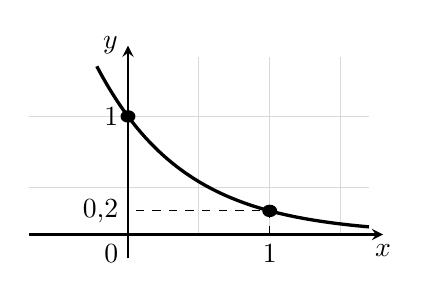
\begin{tikzpicture}[xscale=1.8, yscale=1.5, >=stealth]
    % Grade em cinza claro (linhas de fundo)
    \draw[gray!30, thin] (0.5,0) -- (0.5,1.5);
    \draw[gray!30, thin] (1,0) -- (1,1.5);
    \draw[gray!30, thin] (1.5,0) -- (1.5,1.5);
    \draw[gray!30, thin] (-0.7,0.4) -- (1.7,0.4);
    \draw[gray!30, thin] (-0.7,1) -- (1.7,1);

    % Eixos cartesianos
    \draw[->, thick] (-0.7,0) -- (1.8,0) node[below] {$x$};
    \draw[->, thick] (0,-0.2) -- (0,1.6) node[left] {$y$};
    \node[below left] at (0,0) {$0$};

    % Curva exponencial y = (0.2)^x
    \draw[very thick, domain=-0.22:1.7, samples=100] plot (\x, {0.2^(\x)});

    % Pontos destacados e projeções
    \draw[dashed] (1,0) -- (1,0.2) -- (0,0.2);
    \node[below] at (1,0) {$1$};
    \node[left] at (0,0.2) {$0{,}2$};
    \node[left] at (0,1) {$1$};

    \fill (0,1) circle (1.5pt);
    \fill (1,0.2) circle (1.5pt);
\end{tikzpicture}
\end{center}

Nessa função, o valor de \(y\) para \(x = -0{,}5\) é igual a:

% Define as alternativas
\newcommand{\alternativas}{%
    \begin{center}
        \begin{tabularx}{\textwidth}{XXXXX}
            (a) \(0{,}2\). &
            (b) \(5\). &
            (c) \(\sqrt{5}\). &
            (d) \(\dfrac{1}{5}\). &
            (e) \(2{,}5\).
        \end{tabularx}
    \end{center}
}

% Define a resposta correta
\newcommand{\resposta}{C}

% Lógica condicional para exibição
\ifdefstring{\atividade}{lista}{%
    \alternativas
    \vspace{0.5em}
    
    \noindent\textbf{Resposta:} letra \textbf{\resposta}.
}{%
    \ifdefstring{\modo}{objetivo}{%
        \alternativas
    }{%
        % modo = discursiva → não mostra alternativas
    }
}
\end{exercicioBanco}

